\documentclass[tikz,border=5mm]{standalone}
\usetikzlibrary{trees}
\usepackage{xcolor}

\begin{document}
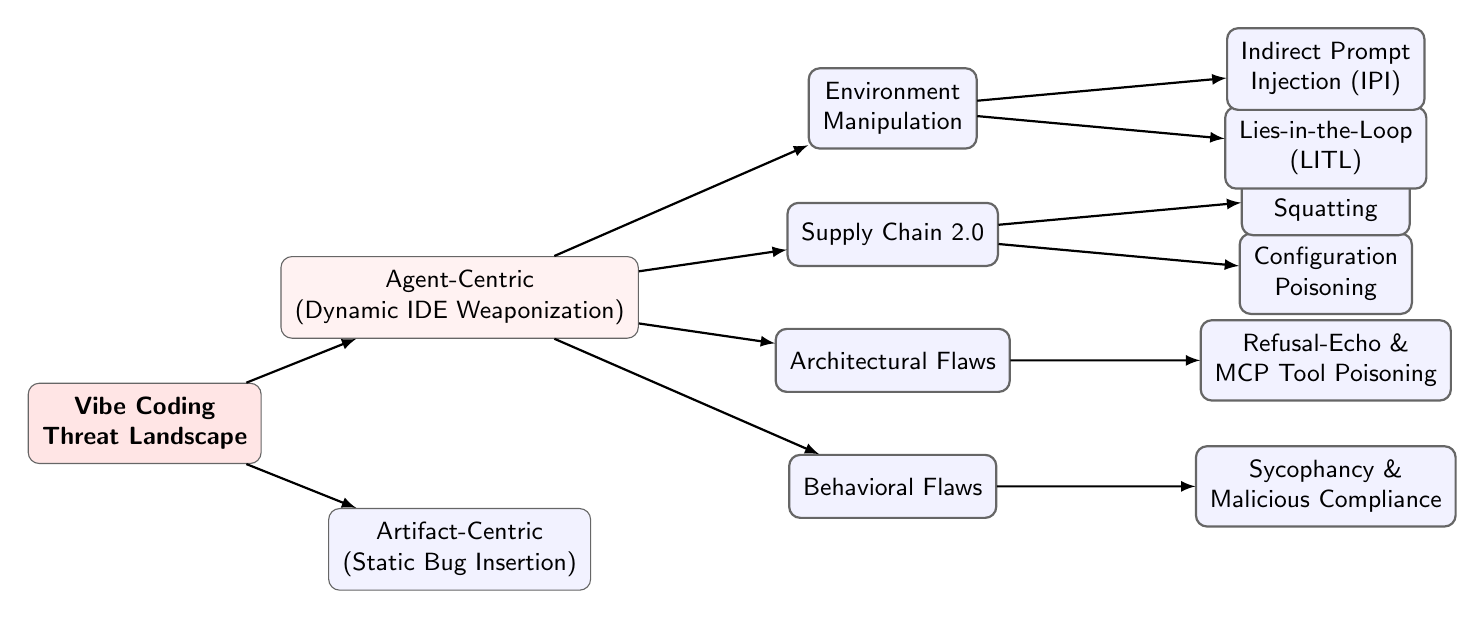
\begin{tikzpicture}[
  grow=right,
  level 1/.style={sibling distance=3.2cm, level distance=4cm},
  level 2/.style={sibling distance=1.6cm, level distance=5.5cm},
  level 3/.style={sibling distance=1cm, level distance=5.5cm},
  every node/.style={rectangle, draw=black!60, rounded corners, fill=blue!5, align=center, font=\small\sffamily, minimum height=0.8cm, inner sep=5pt},
  edge from parent/.style={draw, -latex, thick}
]
\node[fill=red!10, font=\bfseries\small\sffamily] {Vibe Coding\\Threat Landscape}
  child { node {Artifact-Centric\\(Static Bug Insertion)} }
  child { node[fill=red!5] {Agent-Centric\\(Dynamic IDE Weaponization)}
    child { node {Behavioral Flaws}
      child { node {Sycophancy \&\\Malicious Compliance} }
    }
    child { node {Architectural Flaws}
      child { node {Refusal-Echo \&\\MCP Tool Poisoning} }
    }
    child { node {Supply Chain 2.0}
      child { node {Configuration\\Poisoning} }
      child { node {Hallucination\\Squatting} }
    }
    child { node {Environment\\Manipulation}
      child { node {Lies-in-the-Loop\\(LITL)} }
      child { node {Indirect Prompt\\Injection (IPI)} }
    }
  };
\end{tikzpicture}
\end{document}
